\documentclass{article}
\usepackage[utf8]{inputenc}
\usepackage[italian]{babel}
\usepackage{graphicx}
\usepackage{fancyhdr}
\usepackage{lastpage}
\usepackage{hyperref}
\hypersetup{
	colorlinks,
	citecolor=black,
	filecolor=black,
	linkcolor=black,
	urlcolor=blue
}

% Header e footer
\pagestyle{fancy}
\fancyhf{}
\fancyhead[L]{Sushi Nakamura}
\fancyhead[R]{\leftmark}
\fancyfoot[R]{pagina \thepage\ di \pageref{LastPage}}
\renewcommand{\headrulewidth}{1pt}
\renewcommand{\footrulewidth}{1pt}

\begin{document}
	% Frontespizio
	\begin{titlepage}
		\begin{figure}[http]
			\centering
			
\includegraphics[width=6cm]{logo.jpg}
		\end{figure}
	
		\vspace*{2cm}
		
		{\huge\bfseries\centerline{Sushi Nakamura} }
		\centerline{Progetto di Tecnologie Web A.A. 2019/2020}
		
		\vspace*{1cm}
		{\bfseries \centerline{Informazioni sul gruppo}}
		\begin{center}
			\begin{tabular}{ c|l } 
				Membri & Dindinelli Alessandro - XXXXXXX\\ 
				& Frison Nicolò - 1147682\\ 
				& Giardina Mirco - 1136663\\
				& Tommasin Alessandro - 1189293\\ 
			\end{tabular}
		\end{center}
		
		\vspace*{\fill}
		
	\end{titlepage}
	
	% Pagina indici
	\clearpage
	\renewcommand*\contentsname{Indice}
	\tableofcontents	
	\newpage
	
	% Contenuto
	\section{Introduzione}
		\subsection{Abstract}
			Il sito web \textbf{Sushi Nakamura} è stato sviluppato per permettere all'omonimo ristorante di Padova un mezzo per promuovere sè stesso ed il suo nuovo servizio di take away.
			Nel sito è possibile reperire tutte le informazioni riguardanti i contatti ed i prodotti che possono essere acquistati.
			Inoltre l'amministratore ha la possibilità di inserire, rimuovere e modificare eventuali articoli in vendita e news che possono essere visualizzate dagli utenti.
	\section{Analisi}
		\subsection{Analisi dell'utenza}
		\subsection{Casi d'uso}
			I casi d'uso possono essere riassunti sotto le seguenti categorie:
			\subsubsection{Utente non autenticato}
			\subsubsection{Utente generico autenticato}
			\subsubsection{Amministratore}
	\section{Progettazione}
		\subsection{Obiettivi}
		\subsection{Layout}
		\subsection{Accessibilità}
	\section{Implementazione}
		\subsection{Linguaggi}
			\subsubsection{XHTML 1.0 Strict e HTML5}
			\subsubsection{CSS}
			\subsubsection{PHP}
			\subsubsection{SQL}
			Sql è stato usato per codificare il database. Si rimanda al file \textit{creazione\_database.sql} nella cartella \textit{Database} [\href{https://github.com/Mirco469/ProgettoSushi/tree/master/Database}{url}] della repository per il file di costruzione del database. Di seguito il diagramma ER del database:\newline
			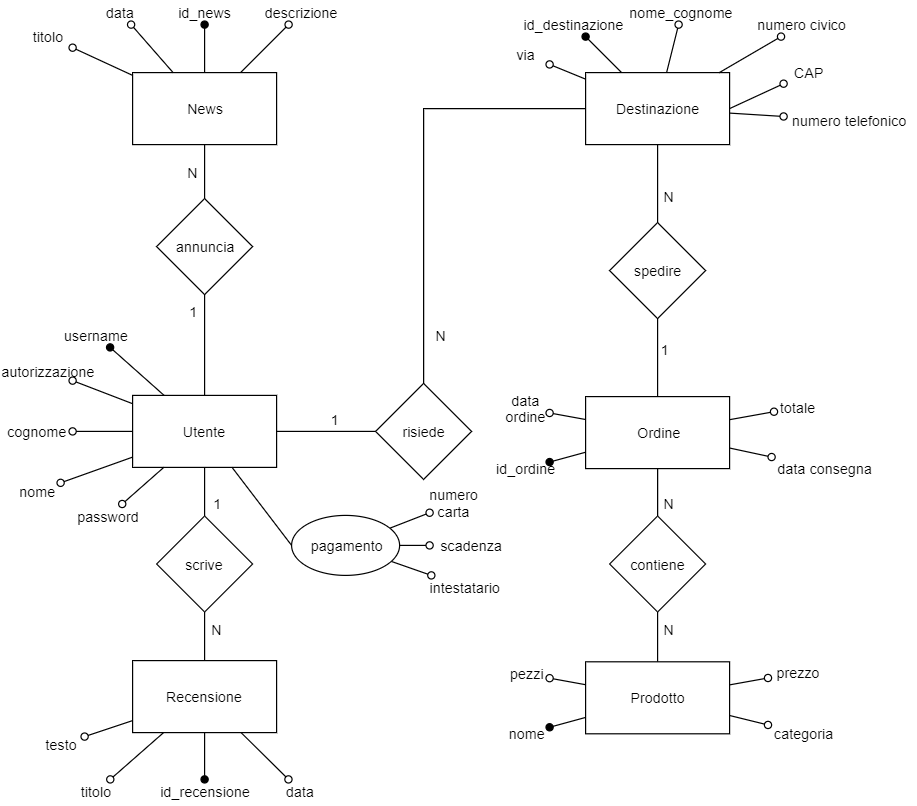
\includegraphics[width=12cm]{DiagrammaER.png}
			\subsubsection{JavaScript}
	\section{Fase di test}
		\subsection{Strumenti usati}
			\subsubsection{W3C HTML Validator}
				Le pagine html sono state validate usando il validatore fornito dall'organizazione W3C per garantire la corretta visualizzazione del contenuto della pagina senza fare entrare i browser in {\bfseries Quirks Mode}. \'E stato usato anche per validare il risultato delle pagine php incollando il risultato ottenuto facendo eseguire lo script php.
			\subsubsection{W3C CSS Validator}
			\subsubsection{TotalValidator}
			\subsubsection{SonarCloud}
				Servizio integrato con GitHub per la verifica del codice nella repository. Ad ogni push veniva fatta un {\bfseries analisi statica} del codice alla ricerca di problemi e vulnerabilità come ad esempio un problema comune è stata la ripetizione rindondate di regole css. Questa fase di test era bloccante, ovvero perchè il codice venisse aggiunto dovevano prima essere risolti i problemi.
	\section{Organizzazione del lavoro}
		Il progetto è stato suddiviso in modo tale che ogni membro avesse la possibilità di creare sia alcune pagine HTML che il relativo CSS, facendo da verificatore nelle pagine degli altri membri.
		Lo stesso può essere detto per quanto concerne PHP, JavaScript e la creazione ed il popolamento del database.
		La sviluppo può essere seguito nella repossitory di GitHub utilizzata:
		\newline
		\newline
		\centerline{ \url{https://github.com/Mirco469/ProgettoSushi}}

\end{document}